\documentclass[tikz, convert=pdf2svg]{standalone}
\usetikzlibrary{positioning, calc, shapes}
\begin{document}
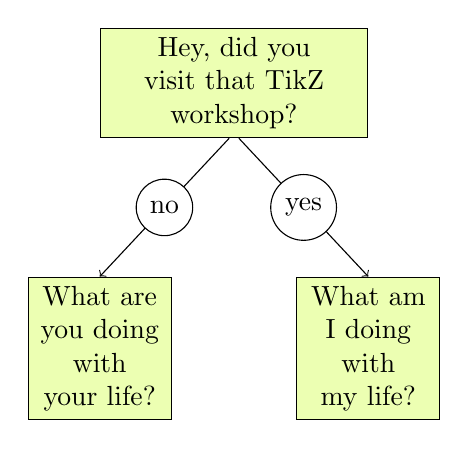
\begin{tikzpicture}
    \node[draw, align=center, text width=90pt, fill=lime!30] (top) {Hey, did you visit that TikZ workshop?};
    
    \node[draw,align=center, text width=45pt, fill=lime!30, below=50pt of top.south west] (no) {What are you doing with your life?};
    \node[draw,align=center, text width=45pt, fill=lime!30, below=50pt of top.south east] (yes) {What am I doing with my life?};

    \draw[->] (top.265) -- (no.north) node[midway, draw, circle, fill=white] {no};
    \draw[->] (top.275) -- (yes.north) node[midway, draw, circle, fill=white] {yes};

\end{tikzpicture}
\end{document}
